	\subsection{Теорема Куммера}

	Начнём с вот такой полезной леммы:

	\begin{lemma}\label{ind_and_p}
		Следующие условия равносильны:
		\begin{enumerate}
			\item $p \not\ \mid \ind(\theta) = |\cO_{K}/\Z[\theta]|$.
			\item $\Z[\theta]/p\Z[\theta] \to \cO_{K}/p\cO_{K}$~--- изоморфизм.
		\end{enumerate}
	\end{lemma}

	\begin{proof}
		Сначала докажем $(2) \implies (1)$. Так как у нас есть изоморфизм $\Z[\theta]/p\Z[\theta] \cong \cO_{K}/p\cO_{K}$, мы имеем 
		\[
			(\cO_k/\Z[\theta])/p(\cO_k/\Z[\theta]) = 0 \implies \cO_k/\Z[\theta] = p\cO_k/\Z[\theta],
		\]
		отукда, так как $|\cO_K/\Z[\theta]| < \infty$, в $\cO_K/\Z[\theta]$ нет элементов $p$-кручения, то есть $p \not \ \mid |\cO_K/\Z[\theta]| = \ind(\theta)$. 

		Теперь докажем $(1) \implies (2)$. Так как $\cO_K/\Z[\theta]$ не имеет $p$-кручения, $\cO_k/\Z[\theta] = p \cO_k/\Z[\theta]$ (у гомоморфизма факторизации тривиальное ядро). Но тогда 
		отображение $\Z[\theta]/(p) \to \cO_K/(p)$~--- эпиморфизм (так как $(\cO_K/(p))/(\Z[\theta]/(p)) \cong (\cO_K/\Z[\theta])/(p) \cong 0$). Но тогда это эпиморфизм векторных пространств над $\F_{p}$ одинаковой размерности (в самом деле, $\Z[\theta] \cong \Z^{n}$ и $\cO_K \cong \Z^n$, где $n = [K : \Q]$). Тогда 
		\[
			\Z[\theta]/(p) \cong \F_{p}^{n} \cong \cO_{K}/(p),
		\]
		как векторные пространства, значит, у нас есть и изоморфизм. 
	\end{proof}

	\begin{theorem}[Куммер]\label{Kummer_theorem} 
		Пусть $K = \Q(\theta)$, $\theta \in \cO_{K}$, а $p$~--- такое простое число, что $p \not \ \mid \ind(\theta)$. Пусть $f$~--- минимальный многочлен $\theta$, причем над полем $\Z/p\Z$ его редукция $\overline{f}$ раскладывается в непривыодимые, как 
		\[
			\overline{f} = \prod_{i} \overline{g_i}^{a_i} \in \F_{p}[t], \ \deg{g_i} = d_i, \ g_i \text{~--- унитарные.}
		\]

		Тогда:
		\vspace{-1mm}
		\begin{enumerate}
			\item Идеалы $\fp_i = (g_i(\theta), p)$~--- все простые идеалы, висящие над простым числом $p$. Причём, они попарно различны. 
			\item $\left\lvert \cO_{K}/\fp_i \right\rvert = p^{d_i}$, а значит, $d_i$~--- степень инерции идеала $\fp_i$.
			\item $p\cO_{K} = \prod \fp_i^{a_i}$, то есть $a_i$ есть индексы ветвления идеалов $\fp_i$.
		\end{enumerate}
 	\end{theorem}
 	\begin{proof}
 		\bf{\RNum{1}.} Покажем, что $\fp_i$ максимальны. Для этого достаточно проверить, что фактор~--- поле. Дейстивтельно, это простое вычисление: 
 		\[
 			\cO_{K}/\fp_{i} = \cO_{K}/(g_i(\theta), p) \underbrace{=}_{\bf{Л.}~\ref{ind_and_p}.} \Z[\theta]/(g_i(\theta), p) \cong \Z[t]/(f(t), p, g_i(t)) \cong \F_{p}[t]/\overline{g_i},
 		\]
 		которое является полем, так как многочлен $g_i$ неприводим над $\F_{p}$. 

 		\bf{\RNum{2}.} Теперь покажем, что $\fp_i \neq \fp_j$ при $i \neq j$. Предположим противное. Тогда 
 		\[
 			\fp_i = \fp_j = (g_i(\theta), p, g_j(\theta)).
 		\]

 		Но, $\overline{g_i}$ и $\overline{g_j}$~--- различные неприводимые многлчлены из $\F_p[t]$, а мы можем линейно представить их НОД: 
 		\[
 			\exists \overline{h_i}, \overline{h_j}\colon \overline{h_i} \overline{g_i} + \overline{h_j} \overline{g_j} = \overline{1} \implies h_i g_i + h_j g_j = 1 + p \cdot q(t) \in \Z[t].
 		\]
 		Подставляя в последнее равенство $\theta$, мы получаем, что $1 \in (g_i(\theta), g_j(\theta), p) = \fp_i = \fp_j$, что противоречит тому, что $\fp_i$ и $\fp_{j}$ максимальны. 

 		\bf{\RNum{3}.} Теперь провреим, что $d_i$~--- степень инерции. Действительно, 
 		\[
 			\cO_{K}/\fp_i \cong \F_{p}[t]/(\overline{g_i}) \implies \left\lvert \cO_{K}/\fp_i \right\rvert = p^{d_i},
 		\]
 		так как $\F_{p}[t]/(\overline{g_i})$~--- расширение $\F_{p}$ степени $d_i$ (так как многочлен $g_i$ неприводим). 

 		Из условия теоремы мы знаем, что 
 		\[
 			f(t) = \prod g_{i}(t)^{a_i} + p h(t) \implies 0 = f(\theta) = \prod g_{i}(\theta)^{a_i} + p h(\theta) \implies   \prod g_{i}(\theta)^{a_i} \in p\cO_{K} \implies \prod \fp_{i}^{a_i} \subset p\cO_{K}.
 		\]

 		Отсюда уже видно, что над $p$ не висит никаких других идеалов. Действительно,  
 		\[
 			p\cO_{K} \subset \fq \implies \prod \fp_i^{a_i} \subset \fq \implies \fp_i \subset \fq \implies \fp_i  = \fq.
 		\]
 		Значит, $\prod \fp_i^{a_i} = p\cO_{K} \cdot I$. Из этого следует, что $a_i \ge e_i$. Остается заметить, что 
 		\[
 			\sum a_i d_i = n, \quad a_i \ge e_i \implies a_i = e_i \forall n. 
 		\]
 	\end{proof}

 	Имеет смысл разобрать полезный частный случай этой теоремы: когда  все $a_i$ равны $1$. 

 	\begin{theorem}\label{Criterion_for_Kummer} 
 		Пусть $K = \Q(\theta), \ \theta \in \cO_{K}$, $f$~--- минимальный многочлен $\theta$, а  $p$~--- простое число. Предположим, что 
 		\[
 		 	\overline{f} = \overline{g_1} \cdot \overline{g_2} \cdot \ldots \cdot \overline{g_k} \in \F_{p}[t], \text{ причем}
 		 \] 

 		 $\overline{g_i}$~--- попарно различые и унитальные.  Тогда $p \not \ \mid \ind(\theta)$.
 	\end{theorem}

 	\begin{proof}
 		 Пусть $I = (p, g_i(\theta)) = I \lei \Z[\theta]$~--- идеал. По тем же соображениям, что и в предыдущей теореме, $I \in \Specm(\Z[\theta])$:
 		 \[
 		 	\Z[\theta]/(g_i(\theta), p) \cong \Z[t]/(f(t), p, g_i(t)) \cong \F_{p}[t]/\overline{g_i}.
 		 \]

 		  Покажем, что $I\cO_{K} \neq \cO_{K}$. Предположим противное и выберем в $\cO_{K}$ целый базис $\omega_1, \ldots, \omega_n$. Тогда мы можем записать каждый элемент базиса с коэффициентами из идеала: 
 		\[
 			\omega_i = \sum a_{i j} \omega_{j}
 		\]
 		Перенося всё в одну часть и обозначая $A = (a_{i j})$, мы имеем такую систему уравнений:
 		\[
 			\lr*{E - A} \cdot \begin{pmatrix} \omega_1 \\ \omega_2 \\ \vdots \\ \omega_n \end{pmatrix} = \begin{pmatrix} 0\\ 0  \\ \vdots \\ 0\end{pmatrix}
 		\]
 		В таком случае $\det{(E - A)} = 0$, из чего следует, что $1 \in I$ (так как $\det(E - a) \in 1 + I$), что противоречит тому, что $I \in \Specm(\Z[\theta])$.

 		Тогда $I\cO_{K}$~--- собственный идеал в $\cO_{K}$, а значит, содержится в некотром максимальном идеале, $(p, g_i(\theta)) \subset \fp_i \subset \cO_{K}$. Теперь нам достаточно показать, что (по лемме \ref{ind_and_p})
 		\[
 		 	\Z[\theta]/(p) \cong \cO_{K}/(p).
 		 \] 
 		 Рассмотрим следующую коммутативную диаграмму: 

 		 \begin{center}
 		 	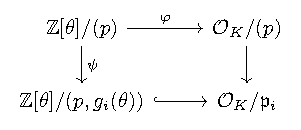
\includegraphics{lectures/4/pictures/cd_1.pdf}
 		 \end{center}

 		 Достаточно проверить, что $\Ker{\varphi} = 0$. Дейстивтельно, пусть $\overline{\alpha} \in \Ker{\varphi}$, тогда $\psi(\overline{\alpha}) = 0$, а значит, $\alpha \in (p, g_{i}(\theta)) \ \forall i$, из чего следует, что 
 		 \[
 		 	\alpha^k \in \prod_{i} (p, g_{i}(\theta)) \in p\Z[\theta] \implies \overline{\alpha}^k = \overline{0} \text{ в } \Z[\theta]/(p),
 		 \]
 		 то есть мы нашли нильпотентный элемент. С другой стороны, 
 		 \[
 		 	\Z[\theta]/(p) \cong \F_{p}[t]/\lr*{\overline{f}} \cong \bigoplus \F_{p}[t]/(\overline{g_i}), 
 		 \]
 		 а то, что написано справа~--- прямое произведение полей. Значит, $\overline{\alpha} = 0$  и ядро тривиально. 
 	\end{proof}

 	\noindent\bf{Ветвление при круговом расширении}

 	Оказывается, теорема Куммера~\ref{Kummer_theorem} позволяет полностью исследовать ветвление при круговом расширении. 

 	Пусть $p$~--- простое число, $K = \Q(\zeta_m)$ и $m \notdivby p$. Как мы знаем, минимальный многочлен $\zeta_m$~--- это круговой многочлен $\Phi_m$. Ясно, что 
 	\[
 		x^m - 1 \divby \Phi_m,
 	\]
 	так как $\Phi_m$~--- минимальный. С другой стороны, многочлен $\overline{x^m - 1}$ имеет $m$ попарно различных корней в $\F_{p}^{alg}$, так как он взаимнопрост со своей производной:
 	\[
 		(x^m - 1, (x^m - 1)') = (x^m - 1, m x^{m - 1}) = 1.
 	\]
 	Но тогда, так как $x^m - 1 \divby \Phi_m$,
 	\[
 		\overline{\Phi_m} = \overline{g_1} \cdot \ldots \overline{g_n},
 	\]
 	где $\overline{g_i}$~--- попарно различные и неприводимые. Тогда по теореме~\ref{Criterion_for_Kummer} $p \not \ \mid \ind(\zeta_m)$, то есть мы можем применить теорему Куммера~\ref{Kummer_theorem}:
 	\[
 	 	p\cO_{K} = \fp_{1} \cdot \ldots \fp_{k}, \quad \fp_{i} = (p, g_i(\zeta_m)). 
 	 \] 

 	 С другой стороны, так как $\Q(\zeta_m)/\Q$~--- расширение Галуа, все степени инерции равны. Значит, достаточно вычислить хотя бы одну. 

 	 \begin{statement} 
 	 	Степени инерции $f$ идеалов $\fp_i$~--- это минимальные такие $f$, что $(p^{f} - 1) \divby m$. 
 	 \end{statement}
 	 \begin{proof}
 	 	Корни многочлена $\overline{x^m - 1}$  образуют циклическую группу, так как это подгруппа в мультипликативной группе конечного расширения $\F_{p}$. Пусть $\theta$~--- образующая этой группы, $\theta \in \F_{p}^{alg}$. 

 	 	\[
 	 		x^m - 1 = \Phi_m(x) \cdot \prod_{k \mid m, k \neq m} \Phi_k(x) \implies \overline{x^m - 1} = \overline{\Phi_m(x)} \cdot \prod_{k \mid m, k \neq m} \overline{\Phi_k(x)}. 
 	 	\]
 	 	Пусть $\Phi_k(\theta) = 0$, тогда так как $x^k - 1 \divby \Phi_k$, $\theta^k - 1 = 0$, откуда $k \divby m$ (так как $\theta$~--- образующая циклической группы из $m$ элементов). Значит, $\overline{\Phi_m} = 0$. 

 	 	Не умаляя общности, пусть $\overline{g_{1}}(\theta) = 0$. Тогда 
 	 	\[
 	 		\{ 1, \theta, \ldots, \theta^{m - 1} \} = \langle \theta \rangle \le \lr*{\F_{p}[x]/(g_1)}^{*}.
 	 	\]
 	 	Тогда, если $\deg{g_1} = f_1$, мы имеем 
 	 	\[
 	 		\left\lvert \lr*{\F_{p}[x]/(g_1)}^{*} \right\rvert = p^{f_1} - 1, \quad \langle \theta \rangle \le lr*{\F_{p}[x]/(g_1)}^{*} \implies p^{f_1} - 1 \divby m,
 	 	\]
 	 	откуда $f_1 \ge f$.  Теперь докажем, что $f_1 \le f$. Действительно, 
 	 	\[
 	 		\begin{cases} \theta^m = 1 \\ m \mid p^{f} - 1 \end{cases} \implies \theta^{p^{f} - 1} = 1 \implies \theta^{p^f} = \theta.
 	 	\]
 	 	Значит, $\theta \in \F_{p^{f}} \implies \F_{p}[x]/(g_1) = \F_{p}[\theta] \le \F_{p^{f}}$, откуда $p^{f} \divby p^{f_1} \implies f_1 \le f$.    
 	 \end{proof}

 	

 		\begin{homework}
 			Задачи:
 			\begin{enumerate}
 				\item Рассмотрим кубическое расщирение $K = \Q(\sqrt[3]{15}) = \Q(\rho)$. 

 				0) Посчитать кольцо $\cO_{K}$.

 				а) Вычислить $\Nm(\rho), \ \Nm(\rho - 1), \ \Nm(\rho + 1), \Nm(\rho - 3)$.

 				б) Докажите, что над простым числом 3 лежит ровно один простой идеал $\rho_3$.

 				в) Докажите, что $\rho_3$~--- главный. Найдите его образующую с помощью разложений $(\rho - 3)$ и $(\rho + 3)$.

 				г) Докажите, что $\frac{9(\rho + 1)^3}{(\rho  - 3)^6}  \in \cO_{K}^{*}$. 

 				\item Вычислить $\cO_{K},$ где $K = \Q(\sqrt{p_1}, \ldots, \sqrt{p_k})$, если $p_i$~--- простые и $p_i \equiv 1 \pmod{4}$.
 				\item  Доказать, что $\upsilon_{\fp}(\cD) \ge e - 1$, где $ e = e(\fp)$~--- индекс ветвления. 

 			\end{enumerate}
 		\end{homework}

 		
 	
